\PassOptionsToPackage{unicode=true}{hyperref} % options for packages loaded elsewhere
\PassOptionsToPackage{hyphens}{url}
%
\documentclass[a4paper,]{article}
\usepackage{lmodern}
\usepackage{amssymb,amsmath}
\usepackage{ifxetex,ifluatex}
\usepackage{fixltx2e} % provides \textsubscript
\ifnum 0\ifxetex 1\fi\ifluatex 1\fi=0 % if pdftex
  \usepackage[T1]{fontenc}
  \usepackage[utf8]{inputenc}
  \usepackage{textcomp} % provides euro and other symbols
\else % if luatex or xelatex
  \usepackage{unicode-math}
  \defaultfontfeatures{Ligatures=TeX,Scale=MatchLowercase}
\fi
% use upquote if available, for straight quotes in verbatim environments
\IfFileExists{upquote.sty}{\usepackage{upquote}}{}
% use microtype if available
\IfFileExists{microtype.sty}{%
\usepackage[]{microtype}
\UseMicrotypeSet[protrusion]{basicmath} % disable protrusion for tt fonts
}{}
\IfFileExists{parskip.sty}{%
\usepackage{parskip}
}{% else
\setlength{\parindent}{0pt}
\setlength{\parskip}{6pt plus 2pt minus 1pt}
}
\usepackage{hyperref}
\hypersetup{
            pdftitle={Ultra Terminum - Invention Details},
            pdfauthor={Max Kaye},
            pdfborder={0 0 0},
            breaklinks=true}
\urlstyle{same}  % don't use monospace font for urls
\usepackage[left=1.5cm,right=1.5cm,top=1.5cm,bottom=1.8cm]{geometry}
\usepackage{longtable,booktabs}
% Fix footnotes in tables (requires footnote package)
\IfFileExists{footnote.sty}{\usepackage{footnote}\makesavenoteenv{longtable}}{}
\setlength{\emergencystretch}{3em}  % prevent overfull lines
\providecommand{\tightlist}{%
  \setlength{\itemsep}{0pt}\setlength{\parskip}{0pt}}
\setcounter{secnumdepth}{5}
% Redefines (sub)paragraphs to behave more like sections
\ifx\paragraph\undefined\else
\let\oldparagraph\paragraph
\renewcommand{\paragraph}[1]{\oldparagraph{#1}\mbox{}}
\fi
\ifx\subparagraph\undefined\else
\let\oldsubparagraph\subparagraph
\renewcommand{\subparagraph}[1]{\oldsubparagraph{#1}\mbox{}}
\fi

% set default figure placement to htbp
\makeatletter
\def\fps@figure{htbp}
\makeatother

\usepackage[utf8]{inputenc}
\usepackage{comment}
\usepackage{siunitx}
\usepackage[lastpage,user]{zref}
%\usepackage{fancyhdr}
\usepackage[dvipsnames]{xcolor}
\usepackage{amsmath, amsfonts}
\usepackage{hyperref}
\usepackage{mdframed}
\usepackage[skins,breakable]{tcolorbox}
\usepackage[yyyymmdd,hhmmss]{datetime}
\usepackage{nicefrac}
\usepackage{epigraph}
\usepackage{verbatim}
\usepackage{subcaption}
\usepackage{float}
\usepackage{xhfill}
\usepackage{varwidth}
\usepackage{pdfpages}
\usepackage{algpseudocode}
\usepackage{algorithm}
\usepackage[toc]{glossaries}
\usepackage{tocloft}
\usepackage[fit]{truncate}
\usepackage{wallpaper}
\usepackage[section]{placeins}

\title{Ultra Terminum - Invention Details}
\author{Max Kaye}
\date{2021-05-08}

\begin{document}
\maketitle

\begin{abstract}
Details of the methods used in Ultra Terminum (UT).
Additionally: details and arguments for UT's novelty, inventiveness, and utility.

UT is a combination of multiple, incremental methods.

The first is \emph{Proof of Reflection}: a method and protocol whereby
a blockchain may utilize an otherwise separate blockchain to
increase its own security and inherit particular security \emph{qualities} of that other blockchain
(which the first blockchain would otherwise never have).
In effect, this is a method for sharing security between blockchains.
If a blockchain uses this method, it does not preclude that blockchain from using it again with another, third blockchain.
Furthermore, this method is universal over all classes of consensus mechanisms that
blockchains may use (e.g., Proof of Work, Proof of Stake, Proof of Authority, etc).

The second is a method for arranging and efficiently operating a set of blockchains using Proof of Reflection to maximize throughput (measured in, e.g., transactions per second), security, and speed.
The result of this method is a construct called \emph{the simplex}.

The third is a method for constructing an unbounded tiling
of simplexes which preserves the security benefits from the second method,
thus providing practically infinite throughput and capacity in a secure environment.

UT claims to solve a well-known problem in the blockchain space, usually called the \emph{scalability trilemma}.
In light of this: the novelty, inventiveness, and utility of UT is somewhat self-evident, as a solution to this problem is highly sought-after.
There is additional reasoning and documentation herein.
\end{abstract}

\begin{section}{Proof of Reflection (PoR)}
    \begin{subsection}{Prerequisites for PoR}
    \end{subsection}
    \begin{subsection}{Required Actions to Facilitate PoR}
    \end{subsection}
    \begin{subsection}{Modification to Existing Consensus Method}
    \end{subsection}
    \begin{subsection}{Method of Operation}
        \autoref{fig:por-step3} illustrates the relationship between blockchains where one of those chains (Chain A) is using the other (Chain B) for reflection.
        Note that these diagrams often simplify the depicted blockchains, in that they produce blocks at a consistent and equal rate.
        In reality, there is no requirement that this holds, and PoR works between any two blockchains regardless of their block production rates and is tolerant of production rates that are inconsistent and/or high variance.
        A demonstration of this tolerance is shown in \autoref{fig:por-with-eth}.

        \begin{figure}[]
            \centering
            \includegraphics[width=.9\linewidth]{../ut/diags/pow_refl_step3_ab_sag}
            \caption{The time-evolution of, and relationship between, two separate blockchains, A and B, where Chain A is using Chain B for PoR.}
            \label{fig:por-step3}
        \end{figure}

        \begin{figure}[]
            \centering
            \includegraphics[width=.9\linewidth]{../ut/diags/por_with_ethereum_sag}
            \caption{The time-evolution of, and relationship between, a blockchain and Ethereum where that first blockchain is using Ethereum as a source of PoR.}
            \label{fig:por-with-eth}
        \end{figure}

    \end{subsection}
    \begin{subsection}{Novelty and Inventiveness}
    \end{subsection}
    \begin{subsection}{Utility}
    \end{subsection}
\end{section}

\begin{section}{Construction of The Simplex}
    \begin{subsection}{Requirements for Participating Blockchains}
        \begin{subsubsection}{Mutual PoR}
            \begin{figure}[H]
                \centering
                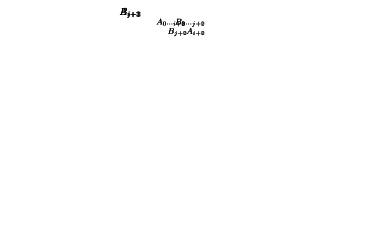
\includegraphics[width=.9\linewidth]{../ut/diags/pow_refl_step5_sag}
                \caption{Relationships between and time-evolution of two blockchains that are mutually reflecting one another.}
                \label{fig:por-step5}
            \end{figure}
        \end{subsubsection}
    \end{subsection}
    \begin{subsection}{Modification to Existing PoR Method}
    \end{subsection}
    \begin{subsection}{Method of Construction}
    \end{subsection}
    \begin{subsection}{Method of Operation}
    \end{subsection}
    \begin{subsection}{Novelty and Inventiveness}
    \end{subsection}
    \begin{subsection}{Utility}
    \end{subsection}
\end{section}

\begin{section}{Simplex Tilings}
    \begin{subsection}{Requirements for Participating Simplexes}
    \end{subsection}
    \begin{subsection}{Modification to Existing Simplex Parameters}
    \end{subsection}
    \begin{subsection}{Method of Construction}
    \end{subsection}
    \begin{subsection}{Method of Operation}
    \end{subsection}
    \begin{subsection}{Novelty and Inventiveness}
    \end{subsection}
    \begin{subsection}{Utility}
    \end{subsection}
\end{section}

\end{document}
